% The adelic solenoid R x Z_2 / Z: strands [0,1) x (a+8Z_2), glued by (1,a) ~ (0,a-1) (generated by a script).
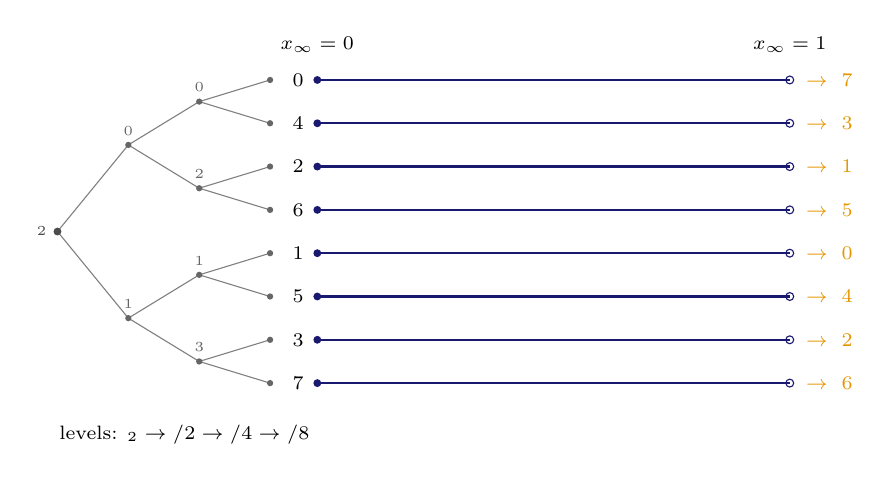
\begin{tikzpicture}[scale=1]
\draw[black!50] (-3.30,-1.925)--(-2.40,-0.825);
\draw[black!50] (-3.30,-1.925)--(-2.40,-3.025);
\draw[black!50] (-2.40,-0.825)--(-1.50,-0.275);
\draw[black!50] (-2.40,-3.025)--(-1.50,-2.475);
\draw[black!50] (-2.40,-0.825)--(-1.50,-1.375);
\draw[black!50] (-2.40,-3.025)--(-1.50,-3.575);
\draw[black!50] (-1.50,-0.275)--(-0.60,0.000);
\draw[black!50] (-1.50,-0.275)--(-0.60,-0.550);
\draw[black!50] (-1.50,-1.375)--(-0.60,-1.100);
\draw[black!50] (-1.50,-1.375)--(-0.60,-1.650);
\draw[black!50] (-1.50,-2.475)--(-0.60,-2.200);
\draw[black!50] (-1.50,-2.475)--(-0.60,-2.750);
\draw[black!50] (-1.50,-3.575)--(-0.60,-3.300);
\draw[black!50] (-1.50,-3.575)--(-0.60,-3.850);
\fill[black!70] (-3.30,-1.925) circle (0.05) node[left,font=\scriptsize]{$\Z_2$};
\fill[black!60] (-2.40,-0.825) circle (0.04) node[above,font=\tiny]{$0$};
\fill[black!60] (-2.40,-3.025) circle (0.04) node[above,font=\tiny]{$1$};
\fill[black!60] (-1.50,-0.275) circle (0.04) node[above,font=\tiny]{$0$};
\fill[black!60] (-1.50,-2.475) circle (0.04) node[above,font=\tiny]{$1$};
\fill[black!60] (-1.50,-1.375) circle (0.04) node[above,font=\tiny]{$2$};
\fill[black!60] (-1.50,-3.575) circle (0.04) node[above,font=\tiny]{$3$};
\fill[black!60] (-0.60,0.000) circle (0.04);
\draw[MidnightBlue,thick] (0,0.000)--(6.00,0.000);
\node[font=\scriptsize,anchor=east] at (-0.05,0.000) {$0$};
\fill[MidnightBlue] (0,0.000) circle (0.05);
\draw[MidnightBlue] (6.00,0.000) circle (0.05);
\node[font=\scriptsize,anchor=west,Orange!90!black] at (6.08,0.000) {$\to\ 7$};
\fill[black!60] (-0.60,-0.550) circle (0.04);
\draw[MidnightBlue,thick] (0,-0.550)--(6.00,-0.550);
\node[font=\scriptsize,anchor=east] at (-0.05,-0.550) {$4$};
\fill[MidnightBlue] (0,-0.550) circle (0.05);
\draw[MidnightBlue] (6.00,-0.550) circle (0.05);
\node[font=\scriptsize,anchor=west,Orange!90!black] at (6.08,-0.550) {$\to\ 3$};
\fill[black!60] (-0.60,-1.100) circle (0.04);
\draw[MidnightBlue,thick] (0,-1.100)--(6.00,-1.100);
\node[font=\scriptsize,anchor=east] at (-0.05,-1.100) {$2$};
\fill[MidnightBlue] (0,-1.100) circle (0.05);
\draw[MidnightBlue] (6.00,-1.100) circle (0.05);
\node[font=\scriptsize,anchor=west,Orange!90!black] at (6.08,-1.100) {$\to\ 1$};
\fill[black!60] (-0.60,-1.650) circle (0.04);
\draw[MidnightBlue,thick] (0,-1.650)--(6.00,-1.650);
\node[font=\scriptsize,anchor=east] at (-0.05,-1.650) {$6$};
\fill[MidnightBlue] (0,-1.650) circle (0.05);
\draw[MidnightBlue] (6.00,-1.650) circle (0.05);
\node[font=\scriptsize,anchor=west,Orange!90!black] at (6.08,-1.650) {$\to\ 5$};
\fill[black!60] (-0.60,-2.200) circle (0.04);
\draw[MidnightBlue,thick] (0,-2.200)--(6.00,-2.200);
\node[font=\scriptsize,anchor=east] at (-0.05,-2.200) {$1$};
\fill[MidnightBlue] (0,-2.200) circle (0.05);
\draw[MidnightBlue] (6.00,-2.200) circle (0.05);
\node[font=\scriptsize,anchor=west,Orange!90!black] at (6.08,-2.200) {$\to\ 0$};
\fill[black!60] (-0.60,-2.750) circle (0.04);
\draw[MidnightBlue,thick] (0,-2.750)--(6.00,-2.750);
\node[font=\scriptsize,anchor=east] at (-0.05,-2.750) {$5$};
\fill[MidnightBlue] (0,-2.750) circle (0.05);
\draw[MidnightBlue] (6.00,-2.750) circle (0.05);
\node[font=\scriptsize,anchor=west,Orange!90!black] at (6.08,-2.750) {$\to\ 4$};
\fill[black!60] (-0.60,-3.300) circle (0.04);
\draw[MidnightBlue,thick] (0,-3.300)--(6.00,-3.300);
\node[font=\scriptsize,anchor=east] at (-0.05,-3.300) {$3$};
\fill[MidnightBlue] (0,-3.300) circle (0.05);
\draw[MidnightBlue] (6.00,-3.300) circle (0.05);
\node[font=\scriptsize,anchor=west,Orange!90!black] at (6.08,-3.300) {$\to\ 2$};
\fill[black!60] (-0.60,-3.850) circle (0.04);
\draw[MidnightBlue,thick] (0,-3.850)--(6.00,-3.850);
\node[font=\scriptsize,anchor=east] at (-0.05,-3.850) {$7$};
\fill[MidnightBlue] (0,-3.850) circle (0.05);
\draw[MidnightBlue] (6.00,-3.850) circle (0.05);
\node[font=\scriptsize,anchor=west,Orange!90!black] at (6.08,-3.850) {$\to\ 6$};
\node[font=\scriptsize] at (0,0.45) {$x_\infty=0$};
\node[font=\scriptsize] at (6.00,0.45) {$x_\infty=1$};
\node[font=\scriptsize,anchor=west,align=left] at (-3.4,-4.50) {levels: $\Z_2\to\Z/2\to\Z/4\to\Z/8$};
\end{tikzpicture}
